\documentclass[11pt, oneside]{article}   	% use "amsart" instead of "article" for AMSLaTeX format


% \usepackage{draftwatermark}
% \SetWatermarkText{Draft}
% \SetWatermarkScale{7}
% \SetWatermarkLightness {0.90} 
%\SetWatermarkColor[rgb]{0.7,0,0}


\usepackage{geometry}                		% See geometry.pdf to learn the layout options. There are lots.
\geometry{letterpaper}                   		% ... or a4paper or a5paper or ... 
%\geometry{landscape}                		% Activate for for rotated page geometry
%\usepackage[parfill]{parskip}    		% Activate to begin paragraphs with an empty line rather than an indent
\usepackage{graphicx}				% Use pdf, png, jpg, or eps� with pdflatex; use eps in DVI mode
								% TeX will automatically convert eps --> pdf in pdflatex		
\usepackage{amssymb}
\usepackage{mathrsfs}
\usepackage{hyperref}
\usepackage{url}
\usepackage{subcaption}
\usepackage{authblk}
\usepackage{amsmath}
\usepackage{mathtools}
\usepackage{graphicx}
\usepackage{fixltx2e}
\usepackage{hyperref}
\usepackage{alltt}
\usepackage{color}
\usepackage[utf8]{inputenc}
\usepackage[english]{babel}
 
\newtheorem{theorem}{Theorem}[section]
\newtheorem{corollary}{Corollary}[theorem]
\newtheorem{lemma}[theorem]{Lemma}

\newcommand{\argmax}{\operatornamewithlimits{argmax}}
\newcommand{\argmin}{\operatornamewithlimits{argmin}}



\title{Report On Layer123 SDN NFV World Congress/NGP Forum\footnote{This report fulfills in full the Stage 1 Deliverable 1 of Project Number HE2017070001.}
Version 1.0}
\author{David Meyer \\
Chief Scientist \\
Huawei Future Network Theory Laboratory \\
dmm@1-4-5.net}

\date{Last update: \today}							% Activate to display a given date or no date


\begin{document}
\maketitle

\section{Introduction} 
\label{sec:intro}
The Layer123 SDN NFV World Congress was helped between October 9-13, 2017 in The Hague, Netherlands and reported roughly 1500 registrants. The ETSI Next Generation Protocols (NGP) Forum was held on October 13, 2017 and was attended by approximately 40 people. The SDN NFV World Congress has grown consistently since I first attended (in 2012) and the trade show part of the Congress was well attended by both exhibitors and delegates (Layer123 calls attendees "delegates").

\bigskip
\noindent
At the highest level, the SDN NFV World Congress was seen as a great success and was attended by a wide variety of key stakeholders.  One easily observable trend was realization that the system disaggregation implied by NFV (and to a lesser extent SDN) will require new and more intelligent forms of automation. Other trends included IoT, AR/VR, and some thinking about how haptic interfaces might work in a 5G environment. Of course, Machine Learning (ML) is the technology that is at the center of these new automation approaches. That said, how exactly ML can help to improve automation is still an open question (and thus a great opportunity). The reason for this is at least two-fold: available data sets and engineering skill sets. Both of these factors will be discussed in more detail in Section \ref{sec:ngp_forum}. The various keynotes and talks can be found here: \url{https://www.layer123.com/sdn-webcast-mle123}.

\bigskip
\noindent
The ETSI NGP Forum was significantly smaller in terms of attendance. However, the Forum still covered a wide variety of topics, including new Internet Protocols (BigIP) designed to meet the challenging requirements of 5G networks,  implementation and experiments of the Recursive InterNetwork Architecture (RINA), Machine Learning for Networking, and Industry 4.0 (the Industrial Internet of Things). These topics will also be reviewed in Section \ref{sec:ngp_forum}.


\bigskip
\noindent
The remained of this report is organized as follows: Section \ref{sec:trends} outlines the trends represented at the Congress and at the NGP Forum. Section \ref{sec:stakeholders} summarizes  my meetings with key stakeholders. Section \ref{sec:ngp_forum} outlines my talk at the NGP Forum and other reflections from the NGP Forum. Finally, Section \ref{sec:conclusions} offers conclusions and recommendations for future work.

\begin{figure}
\center{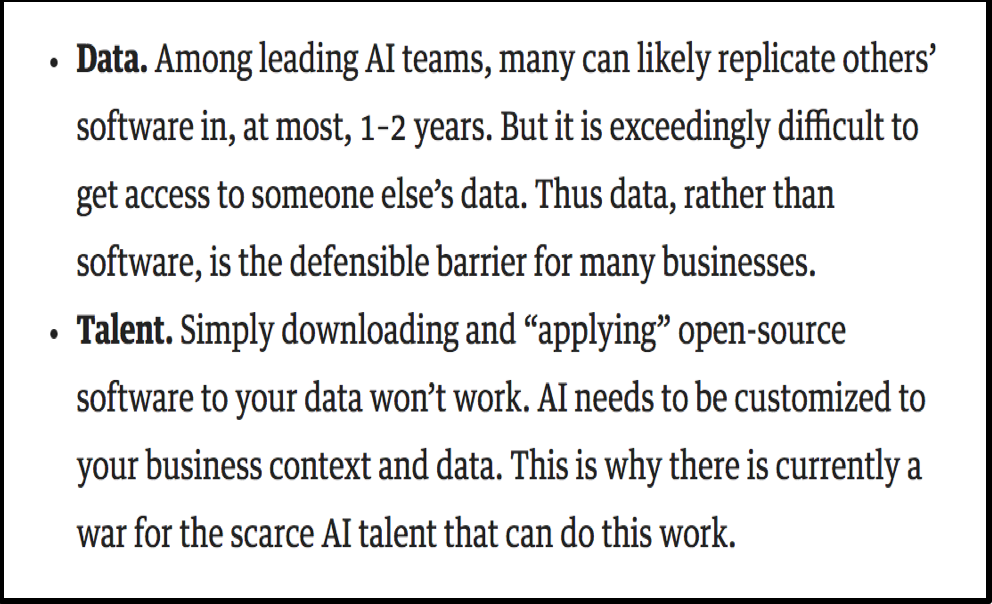
\includegraphics[scale=0.6] {images/talent_data_an.png}}
\caption{Andrew Ng on Data and Talent for Machine Learning. See \\
\url{https://hbr.org/2016/11/what-artificial-intelligence-can-and-cant-do-right-now}}
\label{fig:talent_and_data}
\end{figure}

\section{Trends} 
\label{sec:trends}
The main trends from the Congress can be summarized as follows: Five years after the original NFV proposal \cite{nfv}, we are seeing fully viable deployments that are close to being 100 per cent compliant with the original NFV vision, and we should very soon see a number of operators claim 100 per cent standards compliance. Much of this success has been due to both flexible the open source communities which have enabled NFV to develop quickly. However, we are now seeing that the complexity invoved in the disaggregation that is implied by NFV requires additional intelligence to be viable. Not surprisingly, almost every vendor is marketing some form of "AI" to deal with what we can think of as \emph{disaggregation complexity}\footnote{Here "AI" really means an ad-hoc collection of machine learning techniques.}.

\bigskip
\noindent
Another clearly visible trend is towards programmable pipeline architectures. Barefoot Networks \footnote{\url{https://barefootnetworks.com/}} is clearly in the lead here, and their open source programming language, P4\footnote{\url{https://p4.org/}}, is the current favored way of programming such pipelines. You can see Nick McKeown's keynote on this topic here: \url{ https://www.layer123.com/downloadnow&doc=Stanford_University-1017-McKeown-KEYNOTE}.

\section{Stakeholder Meetings} 
\label{sec:stakeholders}
While I spoke with many people at the Congress, In general there were representatives from the major carriers as well as vendors and users at the event. I have summarized a few of the more interesting conversations I had with key stakeholders below. Nick McKeown is a professor at Stanford University and a founder and Chief Scientist at Barefoot Networks; you might remember Nick as one of the inventors of SDN. Axel  Clauberg is Vice President of Infrastructure at Deutsche Telekom. Michael Howard is an influential analyst at IHS Markit. Prodip Sen is CTO of NFV at HP Enterprise, Diego R. Lopez is a Senior Technology Expert at Telef\'onica, and nd Don Clarke is a Principle Engineer at Cable Labs. I summarize my discussions with each of them below.

\begin{itemize}
\item \textbf{Nick McKeown} \\
I discussed the Intelligence Defined Network (IDN) concepts with Nick in some detail. See Figure \ref{fig:idn_architecture} for a schematic of the IDN architecture. While he had a great deal of interest, we soon started talking about a project in which a Reinforcement Learning (RL) agent could learn a P4 program. I have an action item to pick that up with him in the near future.

\item \textbf{Axel  Clauberg} \\
I spoke with Axel for some time explaining the details of IDN. He has little background in the kinds of mathematics required for successful deployment of machine learning applications at scale (see Figure \ref{fig:talent_and_data}). He outlined how DT, while at the forefront of automating NFV SDN environments, has great need for ML talent (apparently they have few people who can even think about these problems). I agreed to send Axel an email so that we can begin a more substantive discussion about IDN and how it can help DT. That call is scheduled for early December, 2017.


\item \textbf{Michael Howard} \\
Michael is a respected analyst who focuses on emerging technologies for carriers. We discussed IDN in detail, and he wants to interview me for a deeper dive on the topic of Huawei's ML and AI initiatives. This has not been scheduled. Note here: To this end (what is the larger Huawei vision for ML/AI) I am trying to get in touch with the Huawei ML and AI teams (and have spoken with Yanshen about this). However, we haven't yet found a way to make this happen.

\item \textbf{Prodip Sen} \\
Prodip is CTO of NFV Technologies at Hewlett Packard Enterprise (HPE). As such he is very much interested in standardized ML tools to further automate NFV implementations. While very interested in Huawei IDN, he also has very little background in ML and hence the technical aspects of the solution are less compelling. \emph{This suggests that we need a marketing level presentation for people like Prodip}. In any event I took an action item to contact help for a discussion on the fundamentals of ML and how IDN can help automate NFV deployments, as well as making them more "predictive".

\item \textbf{Diego R. Lopez} \\
I have known Diego for many years and we have worked on many projects together. In this discussion we talked
about the ideas behind the IDN architecture, and of course, he was very interested. Telef\'onica has several AI/ML 
initiatives underway\footnote{Apparently including activities with Huawei, but I need to find more information about
exactly what the collaboration is.}, and there is excellent opportunity to further collaborate not only on use cases but
also on the underlying ML technology.

\item \textbf{Don Clarke} \\
Don was a principle at BT focusing on NFV before coming to CableLabs. He has extensive experience in what I would call "old school" automation techniques such as template driven automation (Puppet/Chef, Ansible, etc).  As such, he is very interested in what IDN can bring to NFV both in terms of automation and new capabilities (for example, predictive congestion avoidance).  We informally committed to further discussions. 

\item \textbf{Others} \\
I also spent time with other Huawei employees (such as Sheng Jiang and Renwei Li); as I mentioned above there was a question about the
relationship of BigIP to Active Networking which we discussed. In addition, I spoke with many other people at the meeting but no action items resulted from those interactions
\end{itemize}

\section{NGP Forum} 
\label{sec:ngp_forum}
The NGP Forum (here after Forum) began with Renwei (Richard) Li discussing the charter of the ETSI NGP group. He then talked about what he called BigIP.\footnote{I mentioned to Richard that BigIP looks a lot like \emph{Active Networking} \cite{Tennenhouse:2007:TAN:1290168.1290180} and that we need to be ready to explain the differences.} Next I talked about AI/ML and the IDN concept. While I believe that at some high level the audience understood the concept, the details were clearly beyond most participants. This again suggests that we need a more \emph{marketing oriented} talk/speaker for some parts of events like this. 

\bigskip
\noindent
I talked primarily about two of the IDN use cases: The first use case I talked about was traffic balancing 
using an \emph{actor-critic} architecture for Reinforcement Learning\cite{Sutton:1998:IRL:551283,Lillicrap:2015aa}). 
The basic actor-critc architecture is shown in Figure \ref{fig:ac_architecture}. The second use case was
 SLA/QoS maintenance (using Conditional Variational Auto-Encoders, or CVAEs \cite{NIPS2015_5775}. There 
 was significant interest in both use cases; however, in both cases the actual details of how RL or CVAEs work was 
 really beyond the audience's ability to absorb in the time allotted, which again makes me suggest that a more 
 marketing-oriented approach might have been more appropriate for the venue. 

\begin{figure}
\center{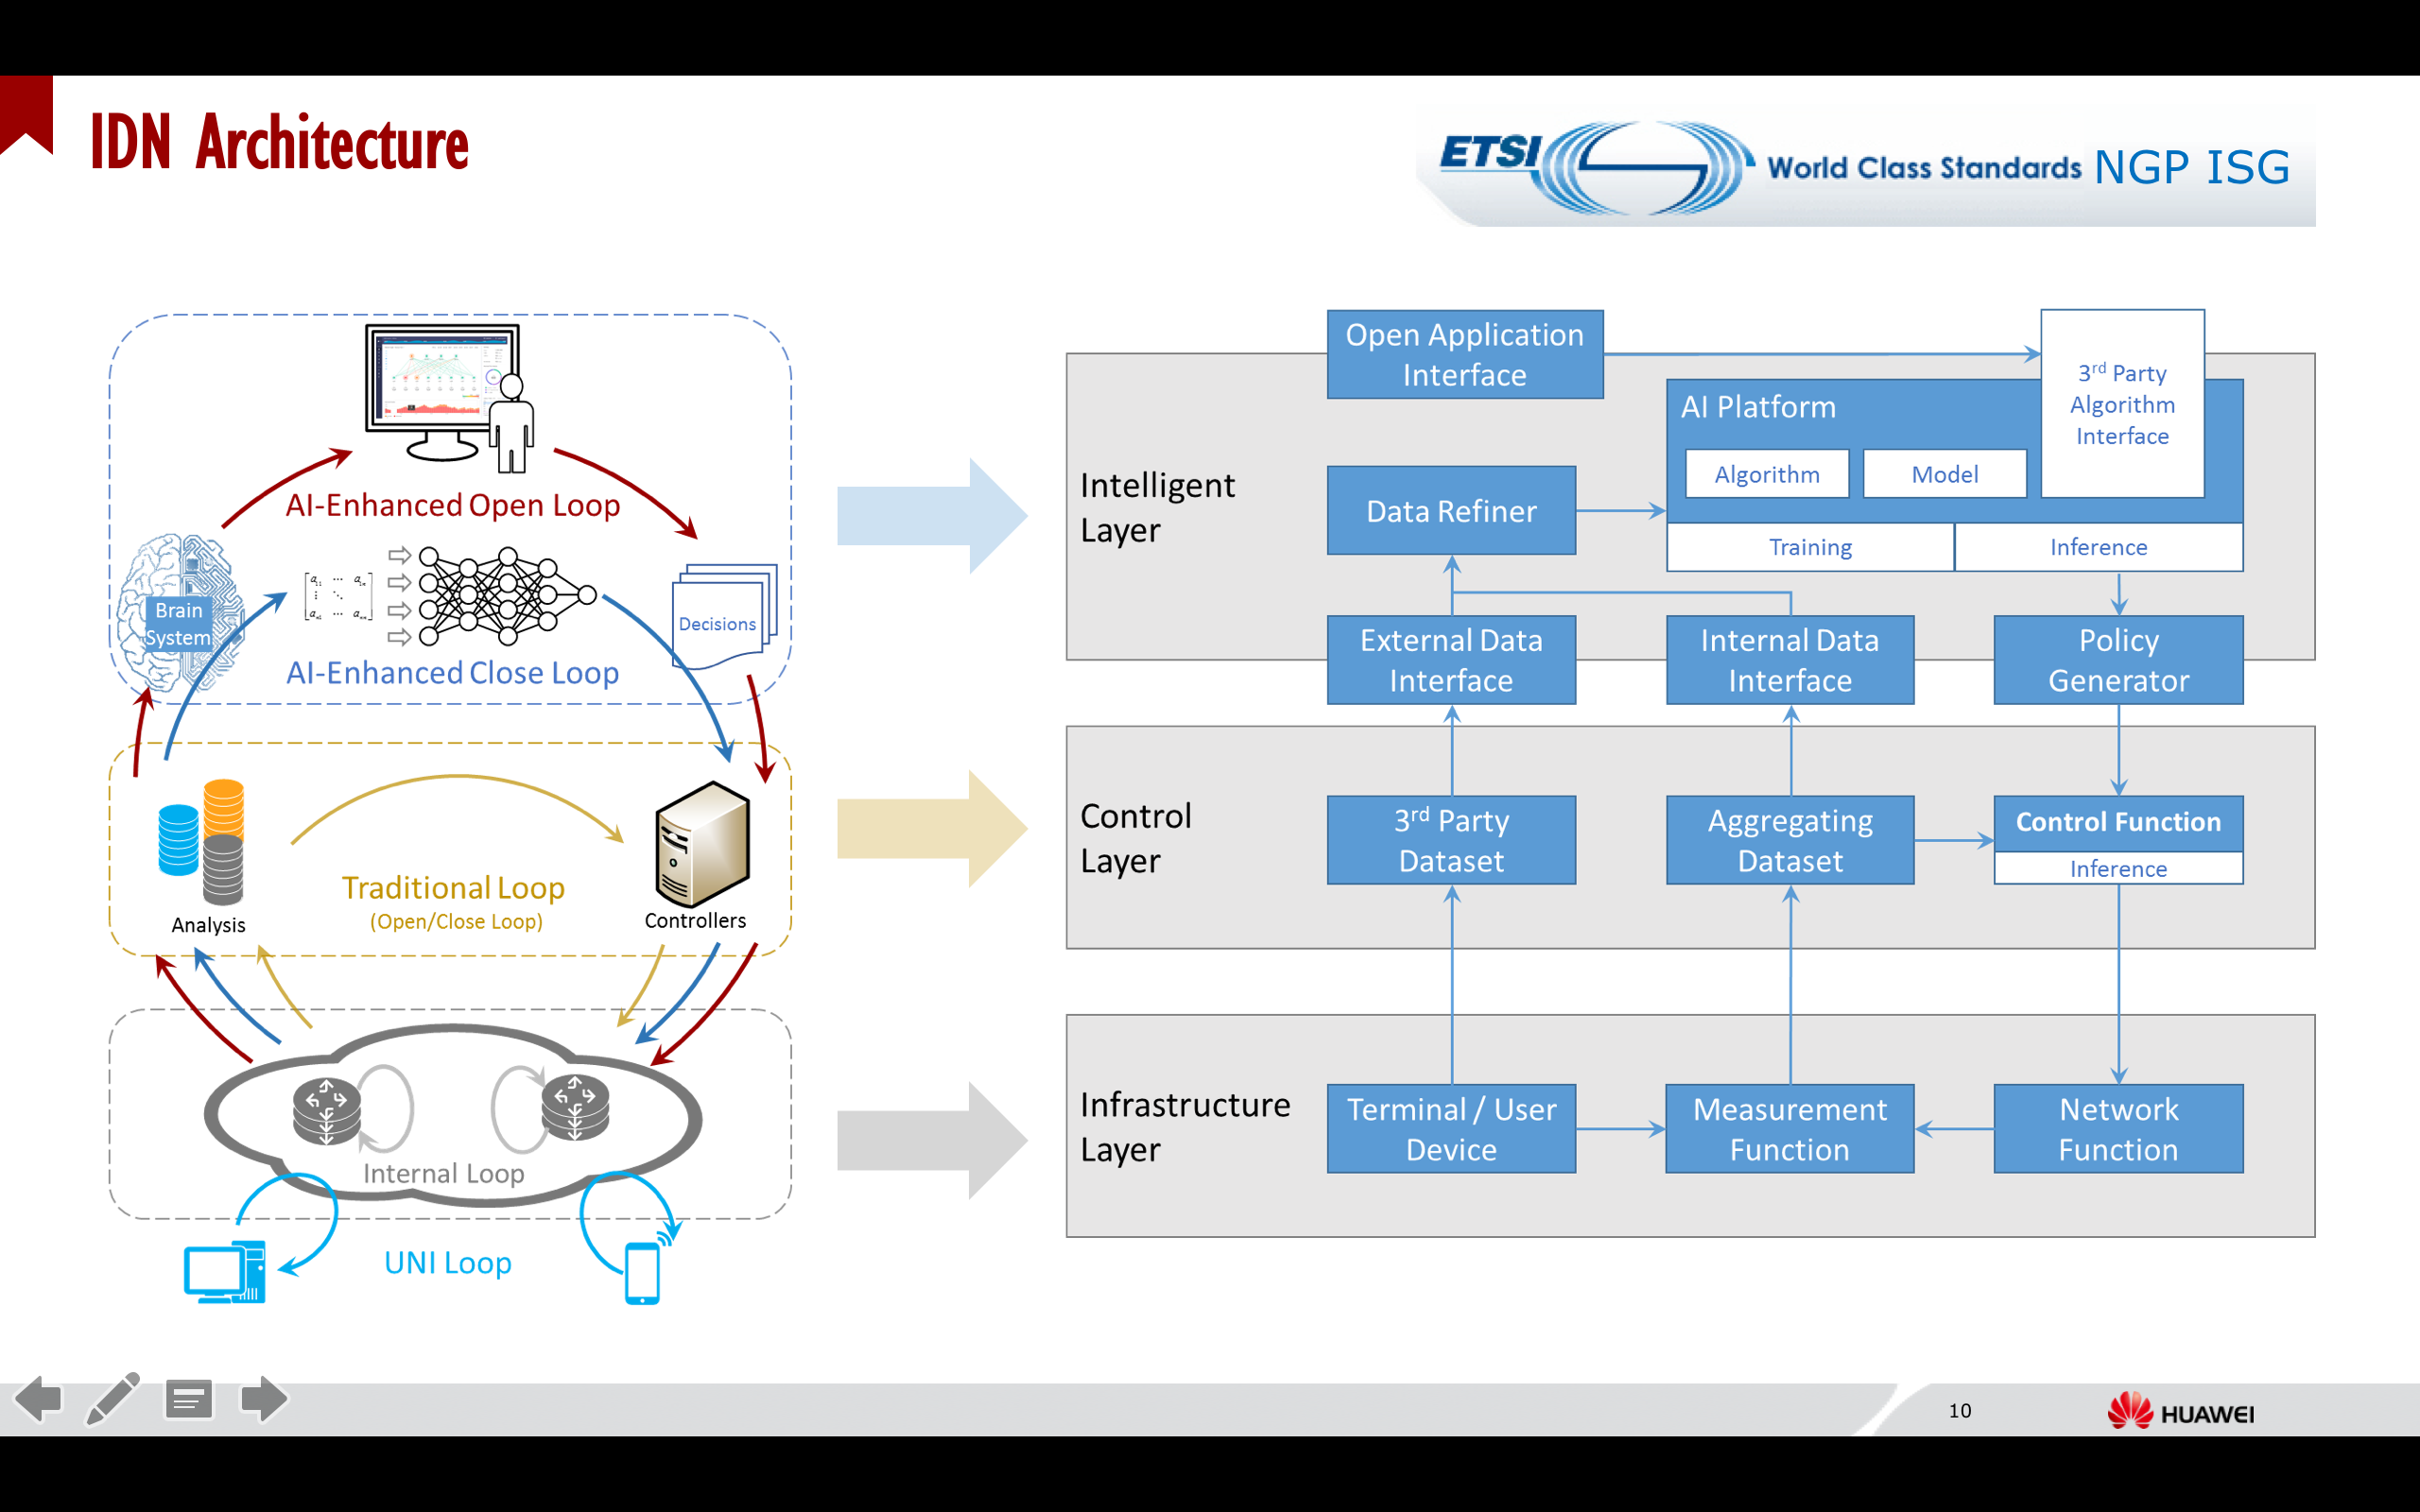
\includegraphics[scale=0.3] {images/idn_architecture.png}}
\caption{Intelligence Defined Network (IDN) Architecture}
\label{fig:idn_architecture}
\end{figure}

\bigskip
\noindent
The next talk, "RINA tales: results from experimental research on a radically simple approach to networking", was given by Eduard Grasa. RINA is a network architecture which owes much to OSI model and is designed by John Day at Boston University. Eduard presented results, but there was little discussion. The next two talks were on the Industrial Internet of Things (IIoT) by Heinrich Munz and Ruediger Kays, respectively, These talks generated some discussion, primarily due to the hard constraints put on the IIoT due to industrial manufacturing requirements. 

\begin{figure}
\center{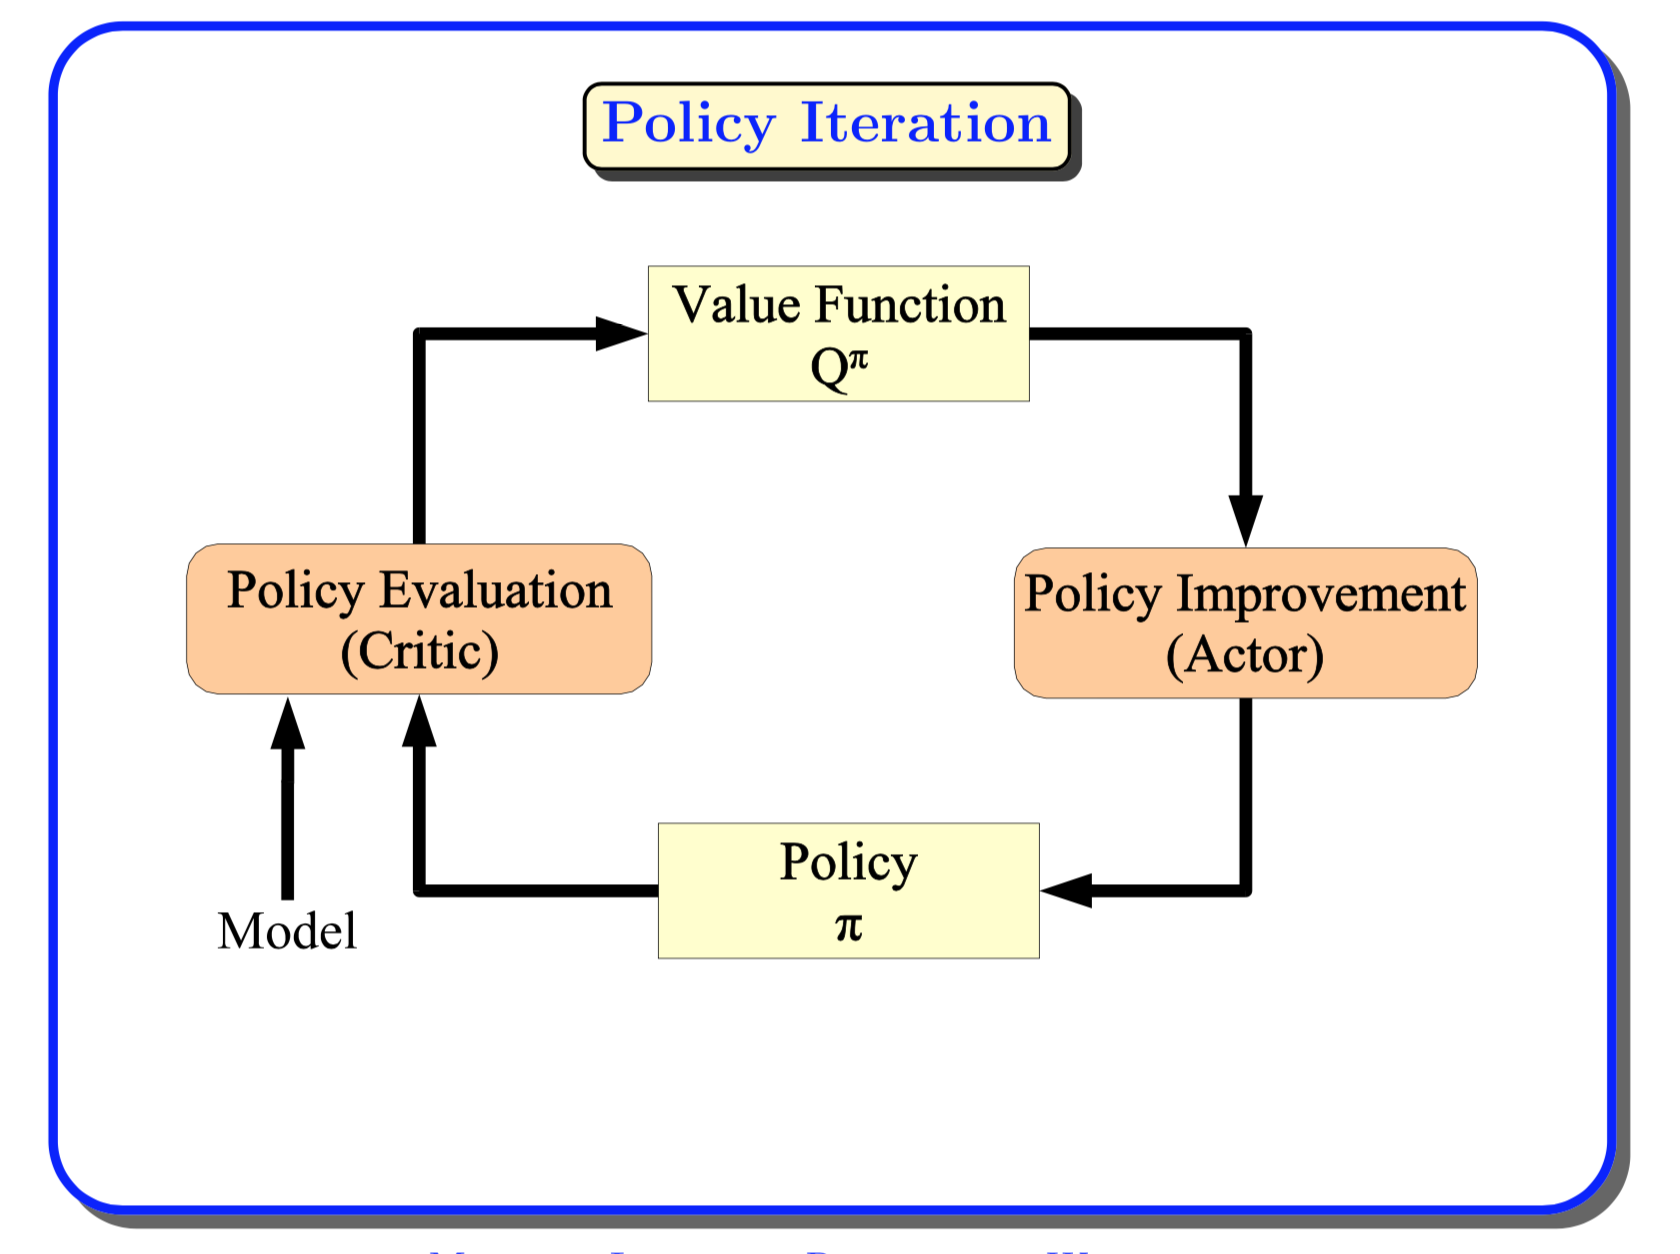
\includegraphics[scale=0.4] {images/ac_architecture.png}}
\caption{Basic Actor-Critic Architecture}
\label{fig:ac_architecture}
\end{figure}


\section{Conclusions and Recommendations} 
\label{sec:conclusions}
There are several takeaways from this meeting. First, the meeting is clearly a worthwhile forum to meet and interact with industry leaders. However, this interaction appears to be primarily on the marketing or "C-level" (executive level), where the actual details of the technologies being discussed are less useful. Again, a more \emph{marketing oriented} approach may be more effective here, especially for technologies like ML which mathematical in nature and hence perhaps more difficult to understand (at least at that level). 

\bigskip
\noindent
The main recommendations of this section can be summarized as follows: First, in the near term we need to provide more detail for the use cases, and to clearly explain the value proposition of each use case. This will also need to be publicized in various venues (see Section \ref{sec:recommendations} below), Second, we need a \emph{theory} of networking into which will unify these ad-hoc approaches; to put in more simply, ad-hoc application of ML techniques 
to the networking domain worn't work. Finally, we need to reach out to a cross-section of the 
management stack so that we can influence at all levels.

\subsection{Recommendations}
\label{sec:recommendations}
\begin{itemize}
\item \textbf{Provide more detail on what exactly IDN is and what its capabilities are} \\
In particular,  how does IDN work (this is essential as IDN must be \emph{explainable} if it is to be adopted by service provides), how does IDN solve existing and future use cases,
and how a theory of network is addressed by IDN.

\item \textbf{Further develop and add to the IDN use cases} \\
The IDN use cases, listed below, need more detail and easy-to-understand examples. The proposed use cases for IDN include:
\begin{itemize}
\item \textbf{Traffic Balancing}\footnote{See Figure \ref{fig:ac} from my NGP Forum talk.}
\begin{figure}
\center{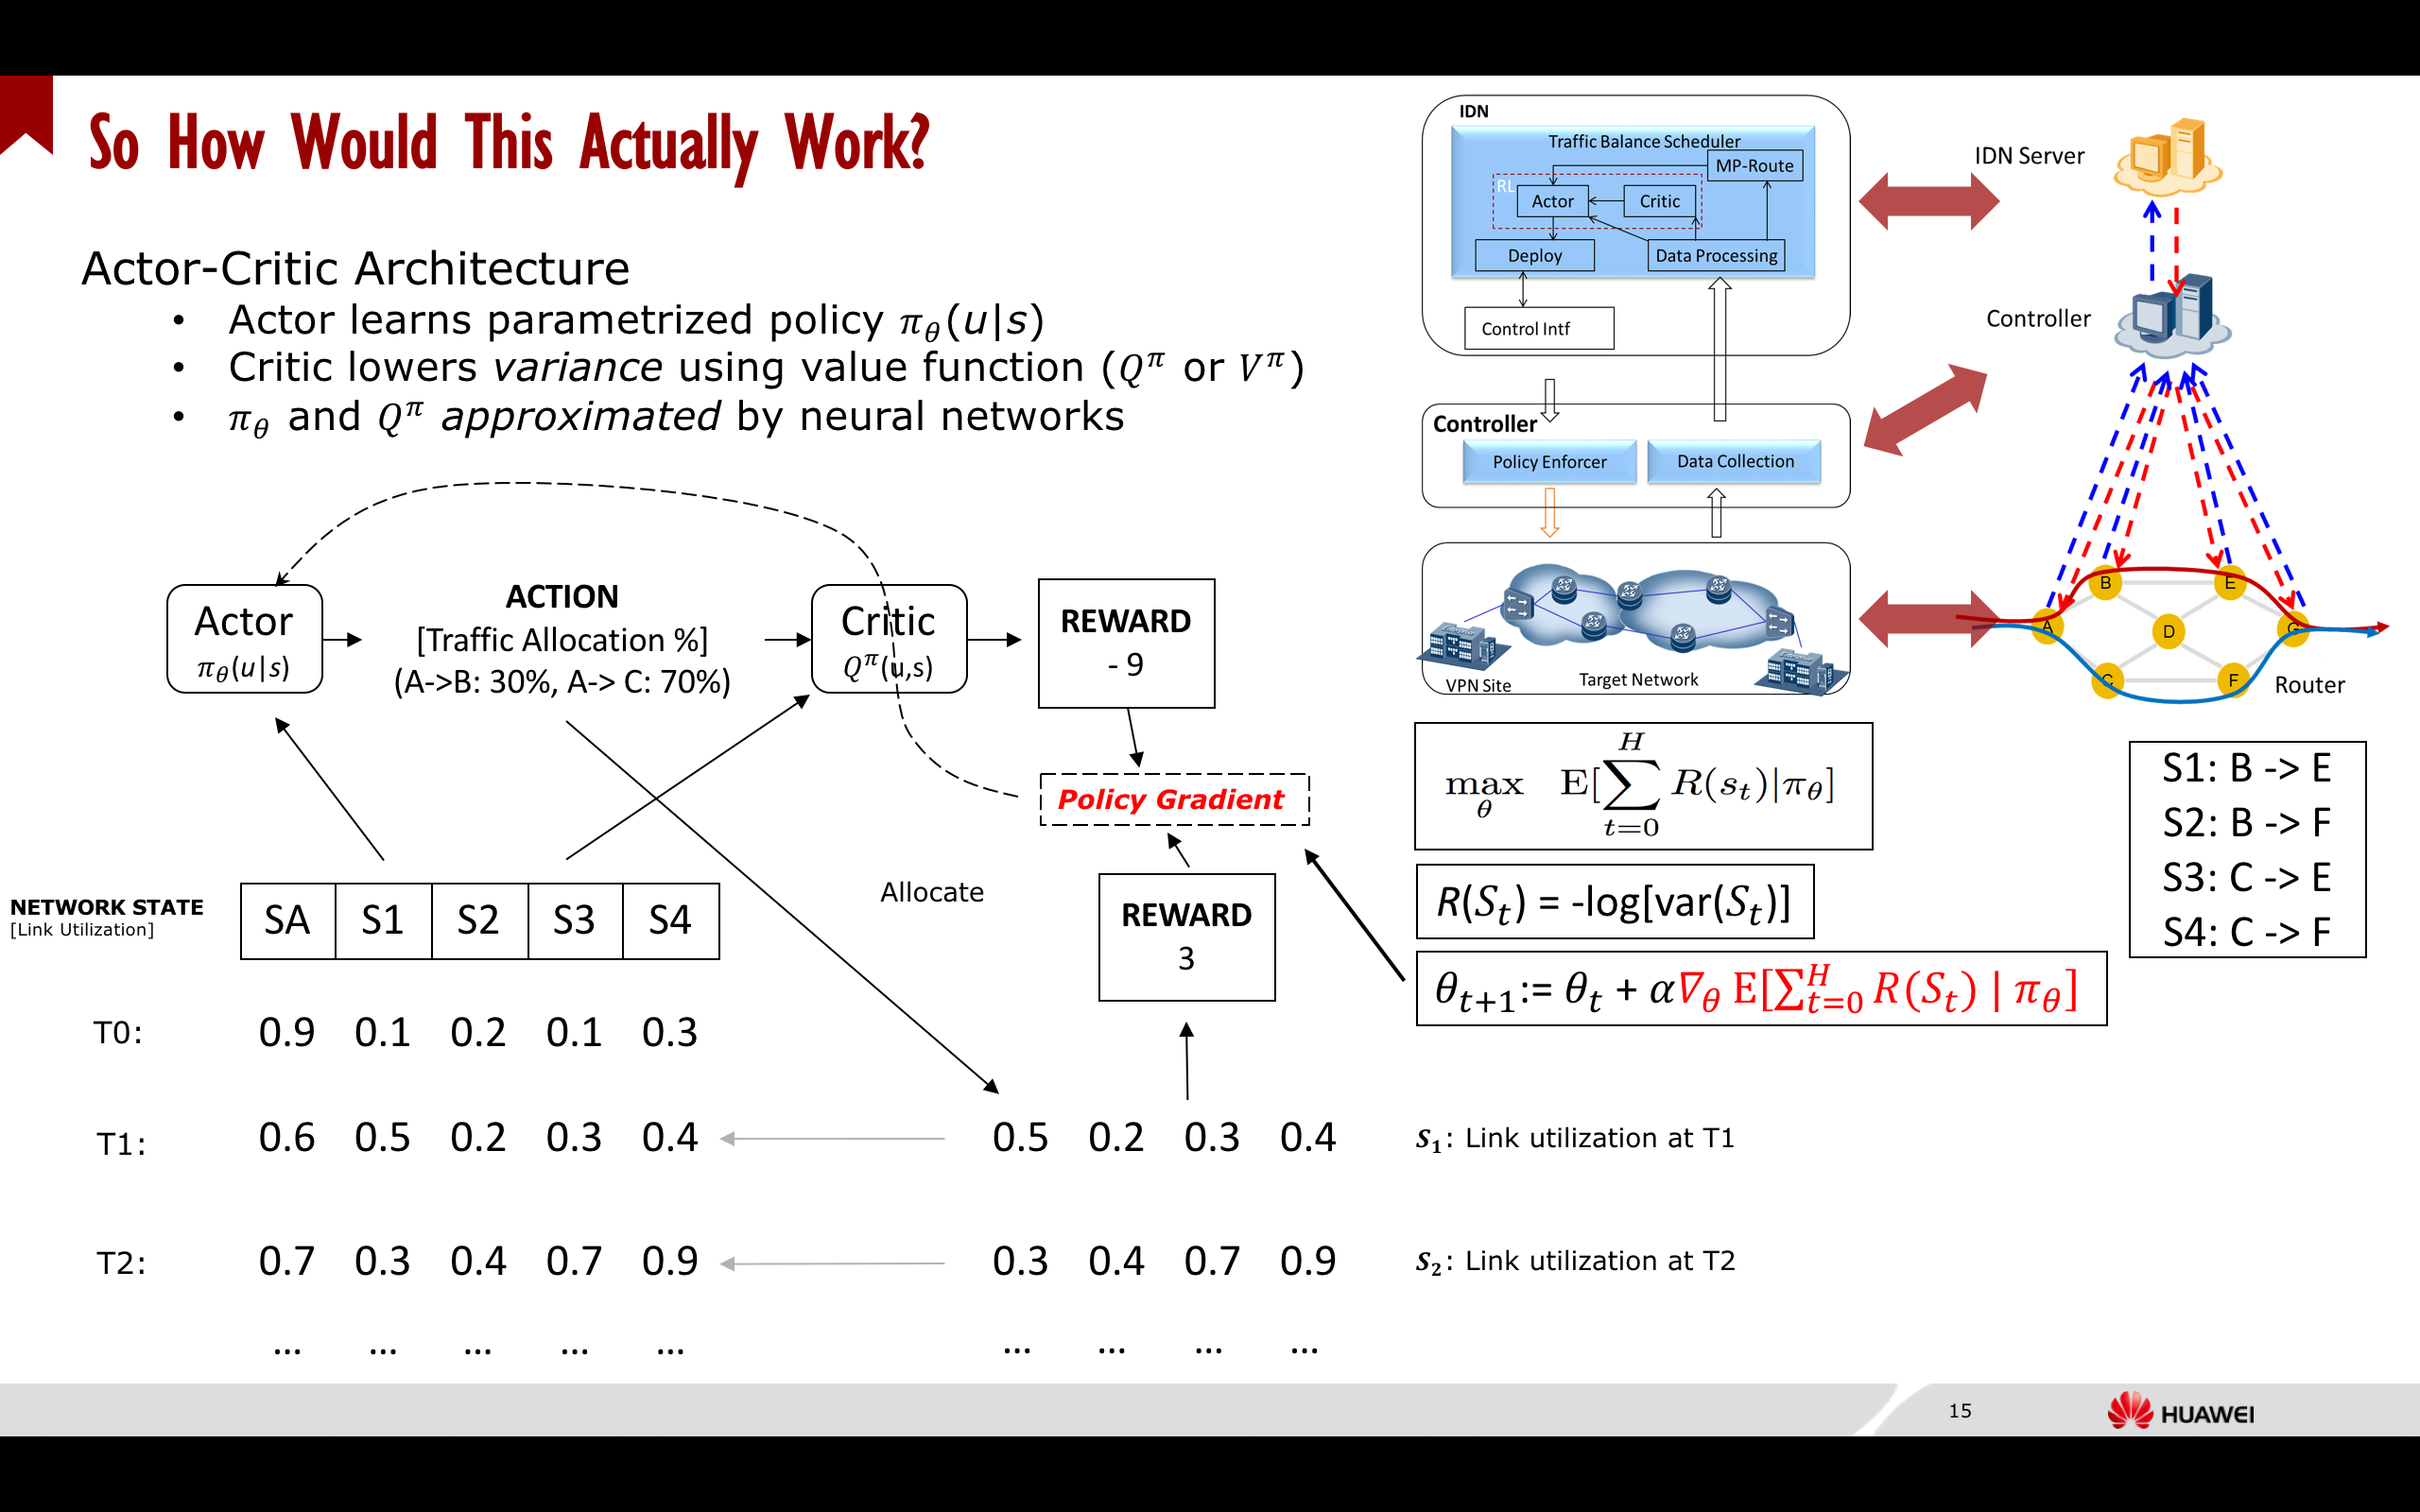
\includegraphics[scale=0.3] {images/ac.png}}
\caption{Actor-Critic Architecture for the Traffic Balancing Use Case}
\label{fig:ac}
\end{figure}

\item \textbf{SLA/QoS Management}\footnote{See Figure \ref{fig:cvae} from my NGP Forum talk.}
\item Overlay/Underlay Traffic Optimization
\item High Throughput TCP 
\item Network Planning
\item Terminal Intelligence
\end{itemize}

\bigskip
\noindent
In addition to these use cases, we need to show how IDN is \emph{extensibile} to new use cases; such use cases could be, for example, from the 5G, NFV, AR/VR. and 
other domains.

\item \textbf{Flesh out the \emph{theory} of Network Intelligence} \\
Most of the "ML for Networking" approaches we see in the market are \emph{ad-hoc} application of known ML techniques to the networking domain. However, there is no unifying theory (or idea) of a network actually is. The work I'm doing with John Doyle\footnote{See \url{http://www.cds.caltech.edu/~doyle/}} at CalTech is intended to fill this gap. We will publish results of integrated control plus learning environments for networking as soon as possible.


\item \textbf{Connect to other ML work in the networking area} \\
There is quite a bit of older work on using ML to solve various problem in the networking space (see, for example  \cite{Tao:2001aa}), 
and with all of the current interest in ML for networking we're seeing new work that attempts to leverage current advancements 
in ML\footnote{see, for example, \cite{Stampa:2017aa}.}.  However, all of this work suffers from the lack of \emph{theory} that I mention above. This theory will need to not only address the fundamental nature of networking but also integrate with ideas of fast and slow control and machine learning. As mentioned above, this theory is the focus of work I am doing with John Doyle at CalTech. This also implies that network engineers must also become facile with machine learning mathematics, concepts, and
implementation.

\begin{figure}
\center{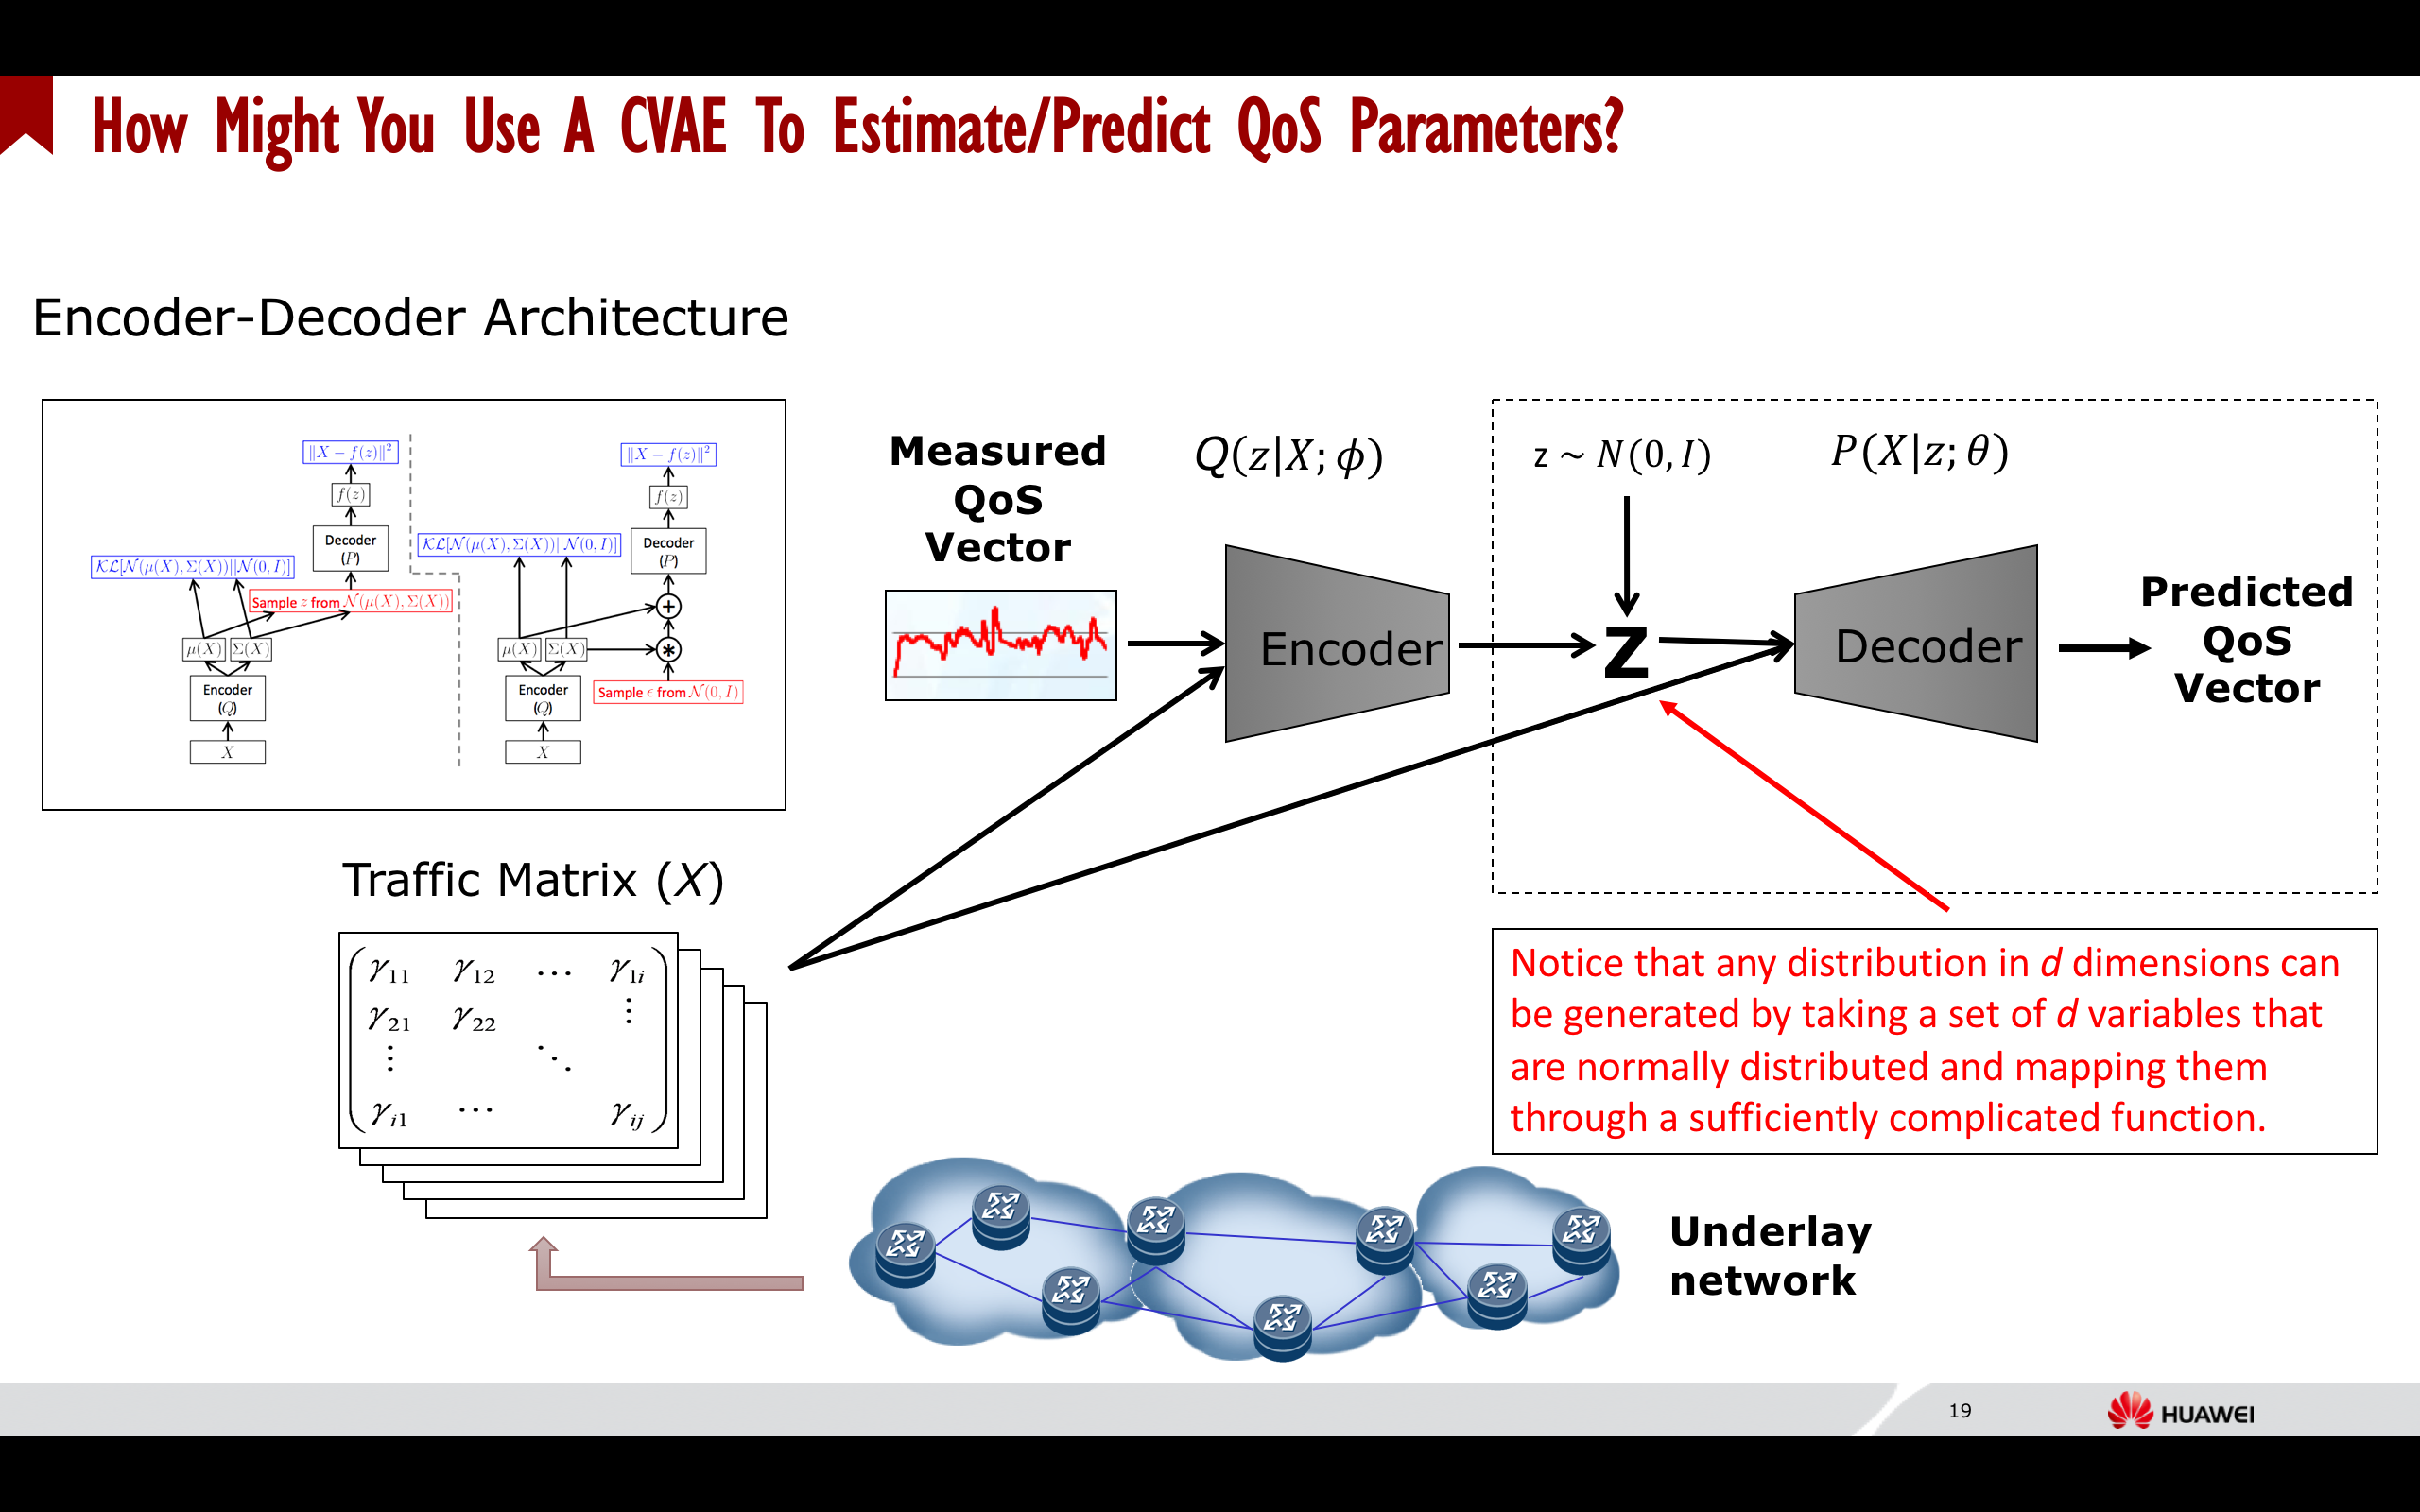
\includegraphics[scale=0.3] {images/cvae.png}}
\caption{Conditional Variational AutoEncoder (CVAE) for the QoS/SLA Use Case}
\label{fig:cvae}
\end{figure}

\item \textbf{Create materials for different groups} 
Different groups require different levels of explanation of both the technology and the associated use cases. These groups include
\begin{itemize}
\item{C-Level}
\item{Network Engineers}
\item{Marketing}
\end{itemize}
Clearly each of these categories require a different level of presentation and different presentation skills. We should develop a set of presentations and presenters that can
address these different categories

\item \textbf{Present IDN at more venuses} \\
These should include not only the typical networking venues (IETF, Layer123, etc) but also to machine learning (e.g., NIPS, ICLR, etc)  and control conferences. These later conference types are of great 
importance as we want to establish leadership in though and innovation.

\item \textbf{Contribute data, source code, and models to public repositories (github)} \\
We (Huawei) should develop guidelines for the release of prototype code, data, and models to our github\footnote{\url{https://github.com/}} repositories. Along with these guidelines, we should have a clear governance model and implementation for what goes into our
public repositories, who can modify these repositories, etc.
\end{itemize}

\bigskip
\noindent
Finally, we need to create deeper connections between the Future Network Theory Laboratory and the work being done in other 
parts of the company in both control and machine learning. For example, we would like to have results in the areas of both control
and learning theory for networking. We also need to get this work into the public as soon
as we have solid results, both in terms of conferences and in public repositories (again, for example \url{https://github.com}).  
To that end I have begun to seek out the appropriate people to facilitate these interactions.

\newpage
\bibliographystyle{ieeetr}
\bibliography{/Users/dmm/papers/huawei/bib/huawei.bib}



\end{document} 
